\begin{minipage}[b]{0.33\linewidth}
\begin{lrbox}{\mybox}%
\begin{lstlisting}[basicstyle=\ttfamily\tiny,escapechar=\%]
;---------------------------------
; Start program at CopyCodeToRAM
; (SYS 2064)
;---------------------------------

* = $0801
 .BYTE $0B,$08
 .BYTE $0A,$00
 .BYTE $9E,$32,$30,$36
 .BYTE $34,$00,$00,$00,$00,$00,$00

;---------------------------------
; CopyCodeToRAM
;---------------------------------
CopyCodeToRAM
 LDA #$40
 STA RAM4000HiPtr
 LDA #$08
 STA RAM0835HiPtr
 LDA #$00
 STA RAM4000LoPtr
 LDA #$35
 STA RAM0835LoPtr
 LDY #$00
 LDX #$06
_Loop   LDA (RAM0835LoPtr),Y
 STA (RAM4000LoPtr),Y
 DEY 
 BNE _Loop
 INC RAM4000HiPtr
 INC RAM0835HiPtr
 DEX 
 BNE _Loop
 JMP InitializeProgram%\index{InitializeProgram}%

NUM_COLS = $28
NUM_ROWS = $18
;------------------------------
; InitializeProgram%\index{InitializeProgram}%
;------------------------------
InitializeProgram%\index{InitializeProgram}%   
 LDA #$00
 STA $D020    ;Border Color
 STA $D021    ;Background Color 0

 LDA #>COLOR_RAM
 STA colorRamHiPtr%\index{colorRamHiPtr}%
 LDA #<COLOR_RAM
 STA colorRamLoPtr%\index{colorRamLoPtr}%

 LDX #$00
_Loop   
 LDA colorRamHiPtr%\index{colorRamHiPtr}%
 STA colorRAMLineTableHiPtrArray%\index{colorRAMLineTableHiPtrArray}%,X
 LDA colorRamLoPtr%\index{colorRamLoPtr}%
 STA colorRAMLineTableLoPtrArray%\index{colorRAMLineTableLoPtrArray}%,X
 CLC 
 ADC #NUM_COLS
 STA colorRamLoPtr%\index{colorRamLoPtr}%
 LDA colorRamHiPtr%\index{colorRamHiPtr}%
 ADC #$00
 STA colorRamHiPtr%\index{colorRamHiPtr}%
 INX 
 CPX #NUM_ROWS+1
 BNE _Loop

 JSR InitializeScreenAndText
 JMP LaunchPsychedelia%\index{LaunchPsychedelia}%

;------------------------------
; InitializeScreenWithInitCharacter%\index{InitializeScreenWithInitCharacter}%
;------------------------------
InitializeScreen   
 LDX #$00
_Loop   
 LDA #$CF
 STA SCREEN_RAM + $0000,X
 STA SCREEN_RAM + $0100,X
 STA SCREEN_RAM + $0200,X
 STA SCREEN_RAM + $0300,X
 LDA #$00
 STA COLOR_RAM + $0000,X
 STA COLOR_RAM + $0100,X
 STA COLOR_RAM + $0200,X
 STA COLOR_RAM + $0300,X
 DEX 
 BNE _Loop
 RTS 

presetColorValuesArray%\index{presetColorValuesArray}%  
  .BYTE BLACK,BLUE,RED,PURPLE,GREEN,CYAN,YELLOW,WHITE
;------------------------------
; LoadXAndYPosition%\index{LoadXAndYPosition}%
;------------------------------
LoadXAndYPosition%\index{LoadXAndYPosition}%   
 LDX pixelYPosition%\index{pixelYPosition}%
 LDA colorRAMLineTableLoPtrArray%\index{colorRAMLineTableLoPtrArray}%,X
 STA curLineInColorRamLoPtr
 LDA colorRAMLineTableHiPtrArray%\index{colorRAMLineTableHiPtrArray}%,X
 STA curLineInColorRamHiPtr
 LDY pixelXPosition%\index{pixelXPosition}%
ReturnEarly
 RTS 

\end{lstlisting}
\end{lrbox}%
\scalebox{0.8}{\usebox{\mybox}}
\end{minipage}
\hspace{-0.1cm}
\begin{minipage}[b]{0.33\linewidth}
\begin{lrbox}{\mybox}%
\begin{lstlisting}[basicstyle=\ttfamily\tiny,escapechar=\%]
;------------------------------
; PaintPixel%\index{PaintPixel}%
;------------------------------
PaintPixel%\index{PaintPixel}%   
 LDA pixelXPosition%\index{pixelXPosition}%
 AND #$80 
 BNE ReturnEarly
 LDA pixelXPosition%\index{pixelXPosition}%
 CMP #NUM_COLS
 BPL ReturnEarly
 LDA pixelYPosition%\index{pixelYPosition}%
 AND #$80 
 BNE ReturnEarly
 LDA pixelYPosition%\index{pixelYPosition}%
 CMP #NUM_ROWS
 BPL ReturnEarly

 JSR LoadXAndYPosition%\index{LoadXAndYPosition}%
 LDA (curLineInColorRamLoPtr),Y
 AND #COLOR_MAX

 LDX #$00
_Loop   
 CMP presetColorValuesArray%\index{presetColorValuesArray}%,X
 BEQ MaybePaintPixel
 INX 
 CPX #COLOR_MAX + 1
 BNE _Loop

MaybePaintPixel   
 TXA 
 STA currentColorValueOfPixel
 LDX colorIndexForCurrentPixel
 INX 
 CPX currentColorValueOfPixel
 BEQ ActuallyPaintPixel%\index{ActuallyPaintPixel}%
 BPL ActuallyPaintPixel%\index{ActuallyPaintPixel}%
 RTS 

ActuallyPaintPixel%\index{ActuallyPaintPixel}%   
 LDX colorIndexForCurrentPixel
 LDA presetColorValuesArray%\index{presetColorValuesArray}%,X
 STA (curLineInColorRamLoPtr),Y
 RTS 

;------------------------------
; PaintStructureAtCurrentPosition%\index{PaintStructureAtCurrentPosition}%
;------------------------------
PaintStructureAtCurrentPosition%\index{PaintStructureAtCurrentPosition}%   
 JSR PaintPixelForCurrentSymmetry%\index{PaintPixelForCurrentSymmetry}%
 LDY #$00
 LDA colorIndexForCurrentPixel
 CMP #$07
 BNE CanLoopAndPaint
 RTS 

CanLoopAndPaint   
 LDA #$07
 STA countToMatchCurrentIndex%\index{countToMatchCurrentIndex}%
       
 LDA pixelXPosition%\index{pixelXPosition}%
 STA initialPixelXPosition
 LDA pixelYPosition%\index{pixelYPosition}%
 STA initialPixelYPosition

PixelPaintLoop%\index{PixelPaintLoop}%   
 LDA initialPixelXPosition
 CLC 
 ADC starOneXPosArray%\index{starOneXPosArray}%,Y
 STA pixelXPosition%\index{pixelXPosition}%

 LDA initialPixelYPosition
 CLC 
 ADC starOneYPosArray%\index{starOneYPosArray}%,Y
 STA pixelYPosition%\index{pixelYPosition}%

 TYA 
 PHA 

 JSR PaintPixelForCurrentSymmetry%\index{PaintPixelForCurrentSymmetry}%

 PLA 
 TAY 
 INY 

 LDA starOneXPosArray%\index{starOneXPosArray}%,Y
 CMP #$55
 BNE PixelPaintLoop%\index{PixelPaintLoop}%

 DEC countToMatchCurrentIndex%\index{countToMatchCurrentIndex}%
 LDA countToMatchCurrentIndex%\index{countToMatchCurrentIndex}%
 CMP colorIndexForCurrentPixel
 BEQ RestorePositionsAndReturn%\index{RestorePositionsAndReturn}%
 CMP #$01
 BEQ RestorePositionsAndReturn%\index{RestorePositionsAndReturn}%

 INY 
 JMP PixelPaintLoop%\index{PixelPaintLoop}%

RestorePositionsAndReturn%\index{RestorePositionsAndReturn}%   
 LDA initialPixelXPosition
 STA pixelXPosition%\index{pixelXPosition}%
 LDA initialPixelYPosition
 STA pixelYPosition%\index{pixelYPosition}%
 RTS 
\end{lstlisting}
\end{lrbox}%
\scalebox{0.8}{\usebox{\mybox}}
\end{minipage}
\hspace{-0.1cm}
\begin{minipage}[b]{0.33\linewidth}
\begin{lrbox}{\mybox}%
\begin{lstlisting}[basicstyle=\ttfamily\tiny,escapechar=\%]
starOneXPosArray%\index{starOneXPosArray}%  
  .BYTE $00,$01,$01,$01,$00
  .BYTE $FF,$FF,$FF,$55 
  .BYTE $00,$02,$00,$FE,$55                 
  .BYTE $00,$03,$00,$FD,$55                 
  .BYTE $00,$04,$00,$FC,$55                 
  .BYTE $FF,$01,$05,$05,$01
  .BYTE $FF,$FB,$FB,$55 
  .BYTE $00,$07,$00,$F9,$55                 
  .BYTE $55                                 
starOneYPosArray%\index{starOneYPosArray}%  
  .BYTE $FF,$FF,$00,$01,$01
  .BYTE $01,$00,$FF,$55 
  .BYTE $FE,$00,$02,$00,$55                 
  .BYTE $FD,$00,$03,$00,$55                 
  .BYTE $FC,$00,$04,$00,$55                 
  .BYTE $FB,$FB,$FF,$01,$05
  .BYTE $05,$01,$FF,$55 
  .BYTE $F9,$00,$07,$00,$55                 
  .BYTE $55                                 
                                            

countToMatchCurrentIndex%\index{countToMatchCurrentIndex}%   .BYTE $01
;------------------------------
; PutRandomByteInAccumulator%\index{PutRandomByteInAccumulator}%
;------------------------------
PutRandomByteInAccumulator%\index{PutRandomByteInAccumulator}%   
randomByteAddress=$414E
 LDA $E199,X
 INC randomByteAddress
 RTS 

 BRK #$00

;------------------------------
; PaintPixelForCurrentSymmetry%\index{PaintPixelForCurrentSymmetry}%
;------------------------------
PaintPixelForCurrentSymmetry%\index{PaintPixelForCurrentSymmetry}%   
 LDA pixelXPosition%\index{pixelXPosition}%
 PHA 
 LDA pixelYPosition%\index{pixelYPosition}%
 PHA 
 JSR PaintPixel%\index{PaintPixel}%

 LDA currentSymmetrySettingForStep%\index{currentSymmetrySettingForStep}%
 BNE HasSymmetry

CleanUpAndReturnFromSymmetry   
 PLA 
 STA pixelYPosition%\index{pixelYPosition}%
 PLA 
 STA pixelXPosition%\index{pixelXPosition}%
 RTS 

 RTS 

HasSymmetry   
 LDA #NUM_COLS
 SEC 
 SBC pixelXPosition%\index{pixelXPosition}%
 STA pixelXPosition%\index{pixelXPosition}%

 JSR PaintPixel%\index{PaintPixel}%

 LDA currentSymmetrySettingForStep%\index{currentSymmetrySettingForStep}%
 CMP #$01
 BEQ CleanUpAndReturnFromSymmetry

 LDA #NUM_ROWS
 SEC 
 SBC pixelYPosition%\index{pixelYPosition}%
 STA pixelYPosition%\index{pixelYPosition}%
 JSR PaintPixel%\index{PaintPixel}%

 PLA 
 TAY 
 PLA 
 STA pixelXPosition%\index{pixelXPosition}%
 TYA 
 PHA 
 JSR PaintPixel%\index{PaintPixel}%
 PLA 
 STA pixelYPosition%\index{pixelYPosition}%
 RTS 

currentSymmetrySettingForStep%\index{currentSymmetrySettingForStep}%
 .BYTE $01
pixelXPositionArray%\index{pixelXPositionArray}%   
 .BYTE $0F,$0E,$0D,$0C,$0B,$0A,$09,$04
 .BYTE $05,$06,$07,$08,$09,$0A,$0B,$0C
 .BYTE $0D,$0E,$0F,$10,$11,$12,$13,$14
 .BYTE $15,$16,$17,$14,$13,$12,$11,$10
 .BYTE $00,$00,$00,$00,$00,$00,$00,$00
 .BYTE $00,$00,$00,$00,$00,$00,$00,$00
 .BYTE $00,$00,$00,$00,$00,$00,$00,$00
 .BYTE $00,$00,$00,$00,$00,$00,$00,$00
pixelYPositionArray%\index{pixelYPositionArray}%   
 .BYTE $0C,$0D,$0E,$0F,$0F,$0F,$0E,$04
 .BYTE $04,$04,$04,$04,$04,$04,$04,$05
 .BYTE $06,$07,$08,$09,$0A,$0B,$0C,$0D
 .BYTE $0D,$0D,$0D,$07,$09,$09,$0A,$0B
 .BYTE $00,$00,$00,$00,$00,$00,$00,$00
 .BYTE $00,$00,$00,$00,$00,$00,$00,$00
 .BYTE $00,$00,$00,$00,$00,$00,$00,$00
 .BYTE $00,$00,$00,$00,$00,$00,$00,$00
\end{lstlisting}
\end{lrbox}%
\scalebox{0.8}{\usebox{\mybox}}
\end{minipage}
\clearpage
\textbf{Lines 1-400. } The first 400 lines or so of the listing opposite
contain the main meat of the painting engine we covered in the previous chapter. In the second
and third columns opposite we find the \icode{PaintPixel\index{PaintPixel}}, \icode{PaintStructureAtCurrentPosition\index{PaintStructureAtCurrentPosition}},
and \icode{PaintPixelForCurrentSymmetry\index{PaintPixelForCurrentSymmetry}} routines, in that order.

The start of the program, in the first columns, contains a number of bookkeeping routines used
at program initialization. You'll note at the very start of the program the clause:
\begin{lstlisting}[escapechar=\%]
* = $0801
\end{lstlisting}
This indicates that the program is loaded to position \icode{\$0801} in RAM. If you imagine the
working memory of the C64\index{C64} as a long tape 65,532 segments long (\icode{\$0000} to \icode{\$FFFF}) then
this little program nestles modestly near the very start of the tape occupying a mere 1415 bytes. So
what you are looking at opposite is approximately 700 or so of these bytes in their assembly language
form.

Near the end of the third column we come to the end of the 'brain' of our truncated version of 
Psychedelia and start into a short section of data. We encountered the use of these arrays in the 
previous chapter and together with the main routines they are responsible for working out what pixels
to paint and where. The hard work is done on the next page, but it is here that the art takes place.

\begin{figure}[H]                                                          
  \centering                                                             
  \begin{adjustbox}{width=8cm,center}                                   
  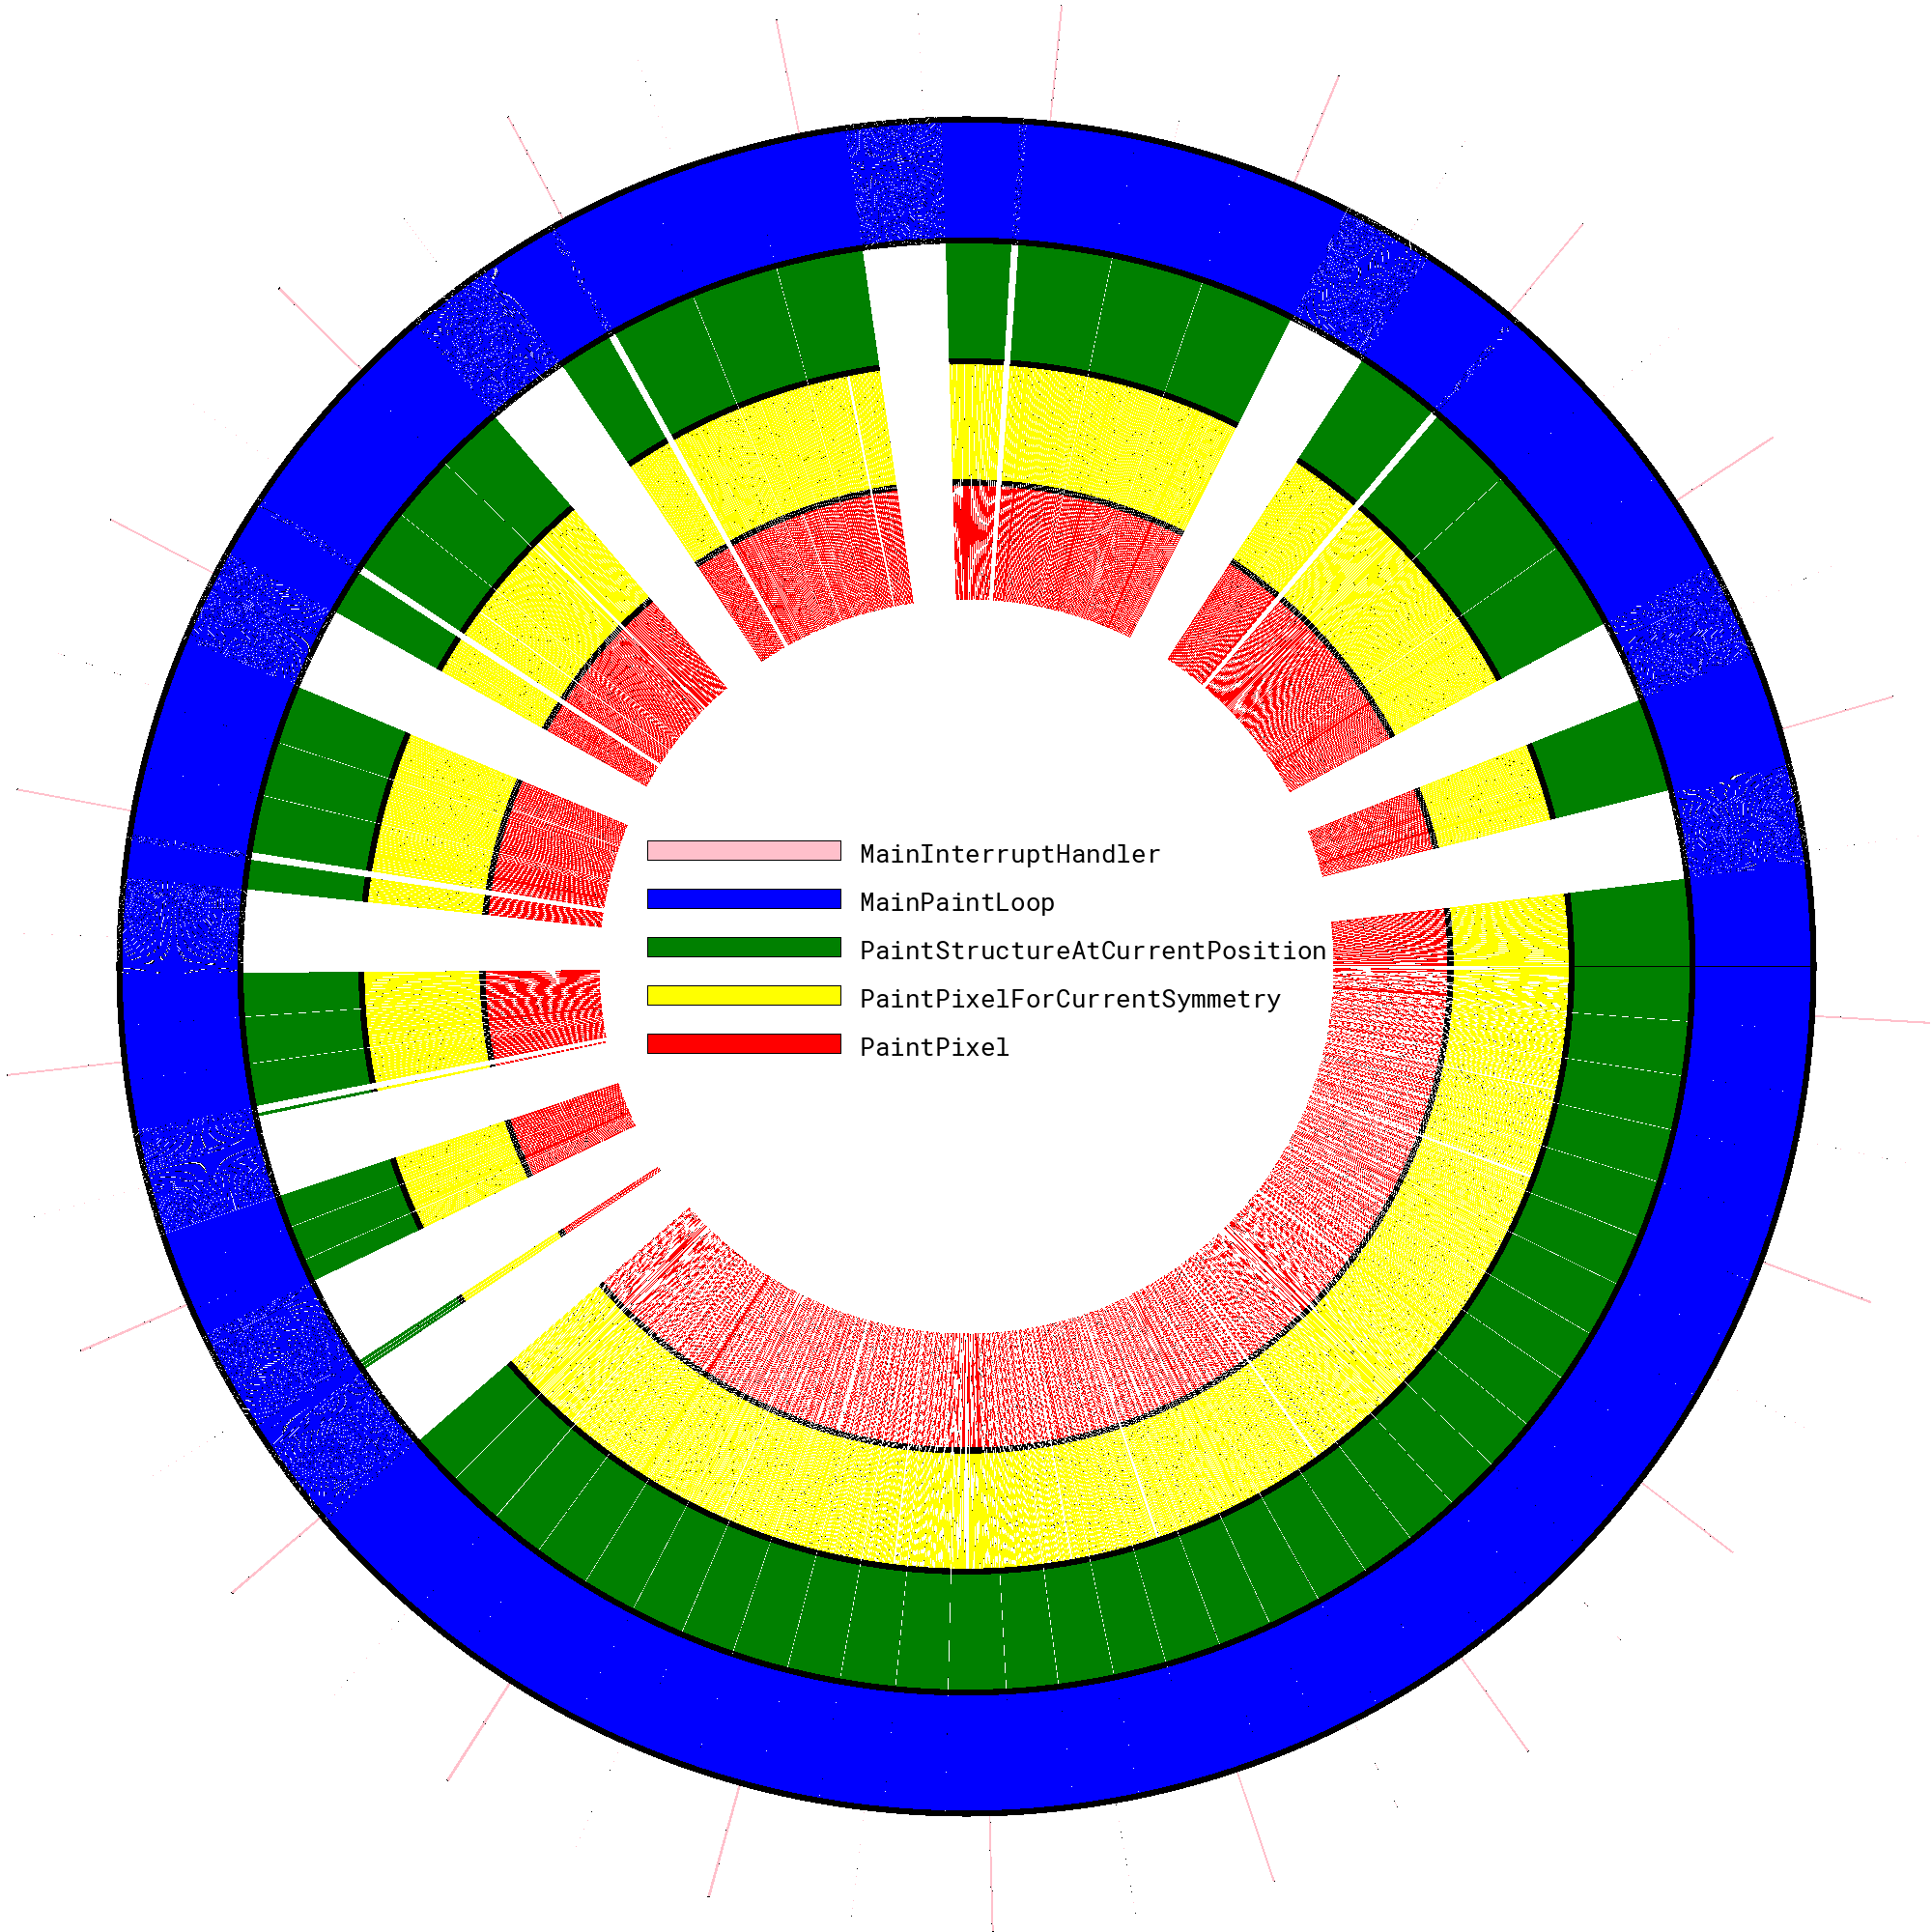
\includegraphics[width=10cm]{src/listing_commentary/execution_cycle_listing.png}%           
  \end{adjustbox}                                                        
\caption{The execution map of a full pattern evolution in the listing edition of Psychedelia.}                                           
\end{figure}                                                               
\clearpage
\begin{minipage}[b]{0.33\linewidth}
\begin{lrbox}{\mybox}%
\begin{lstlisting}[basicstyle=\ttfamily\tiny,escapechar=\%]
currentColorIndexArray%\index{currentColorIndexArray}%   
 .BYTE $FF,$FF,$FF,$FF,$FF,$FF,$FF,$FF
 .BYTE $FF,$FF,$FF,$FF,$FF,$FF,$FF,$FF
 .BYTE $FF,$FF,$FF,$FF,$FF,$FF,$FF,$FF
 .BYTE $FF,$FF,$FF,$FF,$FF,$FF,$FF,$FF
 .BYTE $00,$00,$00,$00,$00,$00,$00,$00
 .BYTE $00,$00,$00,$00,$00,$00,$00,$00
 .BYTE $00,$00,$00,$00,$00,$00,$00,$00
 .BYTE $00,$00,$00,$00,$00,$00,$00,$00

initialFramesRemainingToNext   
 .BYTE $0C,$0C,$0C,$0C,$0C,$0C,$0C,$0C
 .BYTE $0C,$0C,$0C,$0C,$0C,$0C,$0C,$0C
 .BYTE $0C,$0C,$0C,$0C,$0C,$0C,$0C,$0C
 .BYTE $0C,$0C,$0C,$0C,$0C,$0C,$0C,$0C
 .BYTE $00,$00,$00,$00,$00,$00,$00,$00
 .BYTE $00,$00,$00,$00,$00,$00,$00,$00
 .BYTE $00,$00,$00,$00,$00,$00,$00,$00
 .BYTE $00,$00,$00,$00,$00,$00,$00,$00

framesRemainingToNextPaint   
 .BYTE $04,$07,$01,$02,$03,$06,$07,$06
 .BYTE $0C,$02,$03,$06,$07,$01,$02,$02
 .BYTE $04,$04,$07,$01,$02,$03,$06,$07
 .BYTE $0C,$02,$03,$02,$03,$07,$01,$02
 .BYTE $00,$00,$00,$00,$00,$00,$00,$00
 .BYTE $00,$00,$00,$00,$00,$00,$00,$00
 .BYTE $00,$00,$00,$00,$00,$00,$00,$00
 .BYTE $00,$00,$00,$00,$00,$00,$00,$00

;------------------------------
; ReinitializeSequences%\index{ReinitializeSequences}%
;------------------------------
ReinitializeSequences%\index{ReinitializeSequences}%   
 LDX #$00
 TXA 
b42D9   
 STA pixelXPositionArray%\index{pixelXPositionArray}%,X
 STA pixelYPositionArray%\index{pixelYPositionArray}%,X
 STA currentColorIndexArray%\index{currentColorIndexArray}%,X
 STA initialFramesRemainingToNext,X
 STA framesRemainingToNextPaint,X
 INX 
 CPX #$40
 BNE b42D9
 RTS 

;------------------------------
; LaunchPsychedelia%\index{LaunchPsychedelia}%
;------------------------------
LaunchPsychedelia%\index{LaunchPsychedelia}%   
 JSR ReinitializeSequences%\index{ReinitializeSequences}%
 JSR SetUpIntteruptHandlers

;------------------------------
; MainPaintLoop%\index{MainPaintLoop}%
;------------------------------
MainPaintLoop%\index{MainPaintLoop}%   
 INC currentIndexToPixelBuffers%\index{currentIndexToPixelBuffers}%
 LDA currentIndexToPixelBuffers%\index{currentIndexToPixelBuffers}%
 AND maskForFireOffset
 STA currentIndexToPixelBuffers%\index{currentIndexToPixelBuffers}%
 TAX 
 DEC framesRemainingToNextPaint,X
 BNE GoBackToStartOfLoop

 LDA initialFramesRemainingToNext,X
 STA framesRemainingToNextPaint,X

 LDA currentColorIndexArray%\index{currentColorIndexArray}%,X
 CMP #$FF
 BEQ GoBackToStartOfLoop

 STA colorIndexForCurrentPixel
 LDA pixelXPositionArray%\index{pixelXPositionArray}%,X
 STA pixelXPosition%\index{pixelXPosition}%
 LDA pixelYPositionArray%\index{pixelYPositionArray}%,X
 STA pixelYPosition%\index{pixelYPosition}%
 JSR PaintStructureAtCurrentPosition%\index{PaintStructureAtCurrentPosition}%
 LDX currentIndexToPixelBuffers%\index{currentIndexToPixelBuffers}%
 DEC currentColorIndexArray%\index{currentColorIndexArray}%,X
GoBackToStartOfLoop   
 JMP MainPaintLoop%\index{MainPaintLoop}%

;------------------------------
; SetUpInterruptHandlers%\index{SetUpInterruptHandlers}%
;------------------------------
SetUpIntteruptHandlers   
 SEI 
 LDA #<MainInterruptHandler
 STA $0314    ;IRQ
 LDA #>MainInterruptHandler
 STA $0315    ;IRQ

 LDA #$0A
 STA cursorXPosition%\index{cursorXPosition}%
 STA cursorYPosition%\index{cursorYPosition}%

 LDA #$01
 STA $D015    ;Sprite display Enable
 STA $D027    ;Sprite 0 Color
 CLI 
 RTS 

\end{lstlisting}
\end{lrbox}%
\scalebox{0.8}{\usebox{\mybox}}
\end{minipage}
\hspace{-0.1cm}
\begin{minipage}[b]{0.33\linewidth}
\begin{lrbox}{\mybox}%
\begin{lstlisting}[basicstyle=\ttfamily\tiny,escapechar=\%]

currentIndexToPixelBuffers%\index{currentIndexToPixelBuffers}%   .BYTE $08 
stepsToNextInputCheck 
 .BYTE $01
lastColorPainted
 .BYTE $00

;------------------------------
; MainInterruptHandler
;------------------------------
MainInterruptHandler   
 DEC stepsToNextInputCheck
 BEQ b4353
 JMP RETURN_FROM_INTERRUPT

b4353   LDA #$02
 STA stepsToNextInputCheck
 LDA #$00
 STA currentColorToPaint%\index{currentColorToPaint}%

 JSR PaintCursorAtCurrentPosition%\index{PaintCursorAtCurrentPosition}%
 LDA $DC00    ;CIA1: Data Port Register A
 AND #$03
 CMP #$03
 BEQ CheckIfCursorMovedLeftOrRight%\index{CheckIfCursorMovedLeftOrRight}%

 CMP #$02
 BEQ PlayerHasPressedDown

 INC cursorYPosition%\index{cursorYPosition}%
 INC cursorYPosition%\index{cursorYPosition}%

PlayerHasPressedDown   
 DEC cursorYPosition%\index{cursorYPosition}%
 LDA cursorYPosition%\index{cursorYPosition}%
 CMP #$FF
 BNE CheckIfCursorAtBottom

 LDA #$17
 STA cursorYPosition%\index{cursorYPosition}%
 JMP CheckIfCursorMovedLeftOrRight%\index{CheckIfCursorMovedLeftOrRight}%

CheckIfCursorAtBottom   
 CMP #NUM_ROWS
 BNE CheckIfCursorMovedLeftOrRight%\index{CheckIfCursorMovedLeftOrRight}%

 LDA #$00
 STA cursorYPosition%\index{cursorYPosition}%

CheckIfCursorMovedLeftOrRight%\index{CheckIfCursorMovedLeftOrRight}%   
 LDA $DC00    ;CIA1: Data Port Register A
 AND #$0C
 CMP #$0C
 BEQ CheckIfPlayerPressedFire%\index{CheckIfPlayerPressedFire}%

 CMP #$08
 BEQ CursorMovedLeft

 ; Player has pressed right.
 INC cursorXPosition%\index{cursorXPosition}%
 INC cursorXPosition%\index{cursorXPosition}%

CursorMovedLeft   
 DEC cursorXPosition%\index{cursorXPosition}%
 LDA cursorXPosition%\index{cursorXPosition}%
 CMP #$FF
 BNE CheckIfCursorAtExtremeRight

 LDA #$27
 STA cursorXPosition%\index{cursorXPosition}%
 JMP CheckIfPlayerPressedFire%\index{CheckIfPlayerPressedFire}%

CheckIfCursorAtExtremeRight   
 CMP #NUM_COLS
 BNE CheckIfPlayerPressedFire%\index{CheckIfPlayerPressedFire}%
 LDA #$00
 STA cursorXPosition%\index{cursorXPosition}%

CheckIfPlayerPressedFire%\index{CheckIfPlayerPressedFire}%   
 LDA $DC00    ;CIA1: Data Port Register A
 AND #$10
 BEQ PlayerHasntPressedFire

 ; Player has pressed fire.
 LDA #$00
 STA stepsSincePressedFire%\index{stepsSincePressedFire}%
 JMP DrawCursorAndReturnFromInterrupt%\index{DrawCursorAndReturnFromInterrupt}%

PlayerHasntPressedFire   
 LDA stepsExceeded255
 BEQ b43D7
 LDA stepsSincePressedFire%\index{stepsSincePressedFire}%
 BNE DrawCursorAndReturnFromInterrupt%\index{DrawCursorAndReturnFromInterrupt}%

 INC stepsSincePressedFire%\index{stepsSincePressedFire}%
b43D7
 INC seedValueForArrayIndices
 LDA seedValueForArrayIndices
 AND maskForFireOffset
 STA seedValueForArrayIndices

\end{lstlisting}
\end{lrbox}%
\scalebox{0.8}{\usebox{\mybox}}
\end{minipage}
\hspace{-0.1cm}
\begin{minipage}[b]{0.33\linewidth}
\begin{lrbox}{\mybox}%
\begin{lstlisting}[basicstyle=\ttfamily\tiny,escapechar=\%]
UpdateColorIndexArray  
 TAX 
 LDA currentColorIndexArray%\index{currentColorIndexArray}%,X
 CMP #$FF
 BNE DrawCursorAndReturnFromInterrupt%\index{DrawCursorAndReturnFromInterrupt}%

 LDA cursorXPosition%\index{cursorXPosition}%
 STA pixelXPositionArray%\index{pixelXPositionArray}%,X
 LDA cursorYPosition%\index{cursorYPosition}%
 STA pixelYPositionArray%\index{pixelYPositionArray}%,X
 LDA #COLOR_MAX
 STA currentColorIndexArray%\index{currentColorIndexArray}%,X

 LDA smoothingDelay%\index{smoothingDelay}%
 STA initialFramesRemainingToNext,X
 STA framesRemainingToNextPaint,X

DrawCursorAndReturnFromInterrupt%\index{DrawCursorAndReturnFromInterrupt}%   
 JSR LoadXAndYOfCursorPosition%\index{LoadXAndYOfCursorPosition}%
 LDA (curCursorLineColorRamLoPtr),Y
 AND #COLOR_MAX
 STA lastColorPainted
 LDA #WHITE
 STA currentColorToPaint%\index{currentColorToPaint}%
 JSR PaintCursorAtCurrentPosition%\index{PaintCursorAtCurrentPosition}%
 JMP RETURN_FROM_INTERRUPT

;------------------------------
; LoadXAndYOfCursorPosition%\index{LoadXAndYOfCursorPosition}%
;------------------------------
LoadXAndYOfCursorPosition%\index{LoadXAndYOfCursorPosition}%   
 LDX cursorYPosition%\index{cursorYPosition}%
 LDA colorRAMLineTableLoPtrArray%\index{colorRAMLineTableLoPtrArray}%,X
 STA curCursorLineColorRamLoPtr
 LDA colorRAMLineTableHiPtrArray%\index{colorRAMLineTableHiPtrArray}%,X
 STA curCursorLineColorRamHiPtr
 LDY cursorXPosition%\index{cursorXPosition}%
 RTS 

;------------------------------
; PaintCursorAtCurrentPosition%\index{PaintCursorAtCurrentPosition}%
;------------------------------
PaintCursorAtCurrentPosition%\index{PaintCursorAtCurrentPosition}%   
 JSR LoadXAndYOfCursorPosition%\index{LoadXAndYOfCursorPosition}%
 LDA currentColorToPaint%\index{currentColorToPaint}%
 STA (curCursorLineColorRamLoPtr),Y
 RTS 

cursorXPosition%\index{cursorXPosition}%        .BYTE $1E
cursorYPosition%\index{cursorYPosition}%        .BYTE $0D
seedValueForArrayIndices .BYTE $1A
maskForFireOffset      .BYTE $1F
stepsSincePressedFire%\index{stepsSincePressedFire}%  .BYTE $00
stepsExceeded255       .BYTE $00
smoothingDelay%\index{smoothingDelay}%         .BYTE $0C
 .BYTE $00,$00,$00,$00,$00,$00,$00
 .BYTE $5B,$00,$00,$00,$00,$00,$00,$00
 .BYTE $00,$00,$00,$00,$00,$00,$00,$00
 .BYTE $00,$00,$00,$00,$00,$00,$00,$00
 .BYTE $00,$00,$00,$00,$00,$00,$00,$00
 .BYTE $00,$00,$00,$00,$00,$00,$00,$00
 .BYTE $FF,$00,$00,$00,$00,$00,$00,$00
 .BYTE $00,$00,$00,$00,$00,$00,$00,$00
 .BYTE $00,$00,$00,$00,$00,$00,$00,$00
 .BYTE $00,$00,$00,$00,$00,$00,$00,$00
 .BYTE $00,$00,$00,$00,$00,$00,$00,$00
 .BYTE $00,$00,$00,$00,$00,$00,$00,$00
 .BYTE $00,$00,$00,$00,$00,$00,$00,$00
 .BYTE $00,$00,$00,$00,$00,$00,$00,$00
 .BYTE $00,$00,$00,$00,$00,$00,$00,$00
 .BYTE $00,$00,$00,$00,$00,$00,$00,$00
 .BYTE $00,$00,$00,$00,$00,$00,$00,$00
 .BYTE $00,$00,$00,$00,$00,$00,$00,$00
 .BYTE $00,$00,$00,$00,$00,$00,$00,$00
 .BYTE $00,$00,$00,$00,$00,$00,$00,$00
 .BYTE $00,$00,$00,$00,$00,$00,$00,$00
 .BYTE $00,$00,$00,$00,$00,$00,$00,$00
 .BYTE $00,$00,$00,$00,$00,$00,$00,$00
 .BYTE $00,$00,$00,$00,$00,$00,$00,$00
 .BYTE $00,$00,$00,$00,$00,$00,$00

bannerText   
 .TEXT $00,"PSYCHEDELIA...A FORETASTE BY JEFF MINTER"

;------------------------------
; InitializeScreenAndText
;------------------------------
InitializeScreenAndText   
 JSR InitializeScreen

 LDX #NUM_COLS
_Loop   LDA bannerText,X
 STA SCREEN_RAM + $03BF,X
 LDA #$0C
 STA COLOR_RAM + $03BF,X
 DEX 
 BNE _Loop
 RTS 

 .BYTE $00,$00,$00,$BF,$00,$9D,$00,$FF
 .BYTE $00,$FF,$00,$FF,$00,$FF,$00,$DF
 .BYTE $FF,$FF,$FF,$FF,$00

\end{lstlisting}
\end{lrbox}%
\scalebox{0.8}{\usebox{\mybox}}
\end{minipage}
\clearpage
\textbf{Lines 401-720. } This second half of the program contains, towards the bottom of the first column
opposite, the main loop (\icode{MainPaintLoop\index{MainPaintLoop}}) that
runs round and round in a circle for as long as the program itself is running. 

The bulk of the rest of the listing
is what we call an 'interrupt handler', a routine that gets called numerous times every second by the C64\index{C64}
and so is a useful place to do things like checking for user input on the keyboard or joystick, which
is precisely what \icode{MainInterruptHandler} in fact does.

Towards the end, in the third column, we find a couple of helper functions tagged on: \icode{LoadXAndYOfCursorPosition\index{LoadXAndYOfCursorPosition}}
and \icode{PaintCursorAtCurrentPosition\index{PaintCursorAtCurrentPosition}}. These are used by the interrupt handler so can be considered part
of the interrupt handler itself. 

The very last part contains some variables used by the handler, e.g \icode{cursorXPosition\index{cursorXPosition}} and \icode{cursorYPosition\index{cursorYPosition}}.
And then a longish section of unused data, just zero bytes, followed by the text storage for the program's title
screen. We encountered this part in our first chapter, where we saw how the magazine listing had been misprinted
at this point and left us attempting to piece it back together with the program's title as a useful clue for the
missing bytes.

And that is it - a quite tiny program that fits (not quite legibly I'll admit) on just two pages. In the rest of
this chapter we'll dig into the details of each of these routines. It may be useful to refer back here every now
and then to get a sense of where you are on the map as we pull apart the detail.

\clearpage

